\title{Open Sound Controll}
\author{
        Michael Lazarski \\
                Studiengang Media Systems\\
}
\date{\today}
\documentclass[a4paper, 12pt]{article}
\usepackage[ngerman]{babel}
\usepackage[utf8]{inputenc}
\usepackage{graphicx}
\usepackage{float}
\usepackage{url}
\usepackage{hyperref}
\usepackage{textcomp}
\pagestyle{headings}

\begin{document}
\maketitle

\newpage
\tableofcontents
\newpage


\section{Geschichte}
\subsection{Musical Instrument Digital Interface}
Die Geschichte von Open Sound Control beginnt mit MIDI (Musical Instrument Digital Interface).
Also am Anfang der 1980er Große Synthesiyer Manufakturen beginnen MIDI als Standart Protokoll zu Implementieren in ihre Hardware wurde dies damals als eine Revolution in der Musik Industrie angesehen. Nur mit einem Computer, einem Midi Controller und der dazugehöirgen Software konnte ein Musiker aufnehmen, Komponieren und mischen ohne zusätzliches Werkezug. Midi wird bis heute noch in der Musikindustrie benutzt. 
\paragraph{Wie Midi Funktioniert}

MIDI ist eine unidirektionale Schnittstelle zur seriellen Datenübertragung. Midi hat keine Datenflusskontrolle. Die Übertragungsgeschwindigkeit beträgt 31250 Bit/s. \cite{MIDI} \\
\\
Es gibt 3 verschiedene Midi Anschlüsse 
\begin{itemize}
  \item MIDI-IN: Hiermit empfängt der MIDI Controller Signale
  \item MIDI-OUT: Hiermit sendet der MIDI-Controller Signale
  \item MIDI-THRU: Sendet die ankommenden Signale vom MIDI-IN port einfach weiter ohne sie weiter zu verarbeiten
\end{itemize}
 \begin{figure}[htbp]
  \centering
  \fbox{
    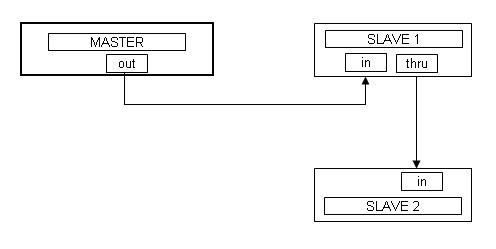
\includegraphics{mms.jpg}
  }
  \caption[MIDI Master Slave \cite{MMS}]{MIDI Master Slave} 
  \label{fig:mms}
\end{figure}
Midi funktioniert nach einem Master-Slave-Prinzip ~\ref{fig:mms}.
Will man mit einem Midi-Keyboard(Master) einen Synthesizer(Slave) steuern, so verbindet man die MIDI-OUT Buchse des Masters mit der MIDI-IN Buchse des Slaves. Möchte man nun noch einen zweiten Slave hinzufügen so schließt man ein Kabel zwischen dem MIDI-THRU des ersten Slaves mit der MIDI-IN Buchse des zweiten Slaves.

\subsubsection{Nachteile von MIDI}
MIDI hat ein paar sehr frustrierende Nachteile:
\begin{itemize}
  \item Serieller transport der Daten. Die Daten müssen erst Sequentiel geordnet werden.
  \item Langsame übertragungs raten. Sehr Problemantisch bei großen Datenmengen.
  \item Pitch wird in Integern dargestellt.
  \item Tendiert zu Keyboard Conrtolleren da Wind, Gittaren und andere Instrumente schwer zu Implementieren sind.
  \item Integer representation von Controller values. Dies kann zu ungenauigkeit führen beim einstellen von feinen paramtern.
  \item Ungenau Zeitauflösung. Diese wird auch wieder in Integern angegeben.
  \item MIDI benötig Spezielle Hardware. 
\end{itemize}
\subsection {Zeta Instrument Processor Interface}
1994 wurde von der Firma Zeta Instruments und einer Research Gruppe der University of California das Zeta Instrument Processor Interface (kurz ZIPI) vorgestellt. Es sollte MIDI ablössen und war aufdem OSI-Model aufgebaut. ZIPI konnte sich nie wirklich durchsetzen. MIDI hat eine Peer-to-Peer Architektur. ZIPI baute auf eine Stern Architektur mit einem HUB in der Mitte als zentrale Anlaufsstelle. Das hatte den vorteil das man einfach Geräte aus dem HUB entfernen konnte. ZIPI ist auch unabhängig von einer Physikalischen Implementierung. Das alles hat aber nicht geholfen da das Adressierungschema zu komplex war. Es mussten 1016127 Synth zustände geregelt werden im ZIPI Controller. Zum vergleich hatte midi nur 16 Kanäle die zwischen 12 und 128 zuständen hatten.
Es gibt bis heute keine Kommerziel vertriebenen Geräte die ZIPI unterstützen.
\newpage
\section{Open Sound Control}
1997 Kündigten die ZIPI Entwickler Matt Wright und Adrian Freed das Open Sound Protokoll an was mehr bekannt ist unter dem namen Open Sound Controll ist ein gutes beispiel von modernen netzwerk datenüberagungs Kontroll Systemen. Wie andere Transport Protokolle erlaubt Open Sound Controll es das die Kommunikation zwischen einem Computer und anderen Medien Geräten statfinden kann, darüber hinaus ermöglicht Open Sound Controll auch die möglichkeit das Programme die auf einem Gerät laufen Daten miteinander austauschen können. Open Sound Control wurde speziell für Musiker entwickelt es kann aber auch gut in anderen gebieten der Netzwerk basierten Kontrolle von System angewendet werden.

\subsection{Technik}
Einer der vorteile von Open Sound Controll ist das man dafür keine Spezielle Hardware braucht wie es z.B. bei MIDI der Fall ist. Open Sound Controll untersützt das Transmission Control Protocol kurz TCP und das User Datagram Protocol kurz UDP, die allgemein bekannt sind und z.B. im Internet oder im Heimnetzwerk schon verwendet werden. Dadurch hat Open Sound Control keine Geschwindigkeitsgrenze. Wir das Netzwerks chneller in dem Open Sound Control eingesetzt wird schneller so wird auch das Proktoll schneller verarbeitet. Durch diese Architektur könnte man Open Sound Control auch Open Stuff Control nennen da theoretisch damit alles gesteuert werden kann was eine Netzwerkschnittstelle hat.

\subsubsection{Transmission Control Protocol}
TCP ist ein verbindungsorientiertes Protokoll. Das heisst jeder Teilnehmer eines Netzwerkes kann exakt zurück verfolgt werden. Der direkte Austausch zweier Stellen ist gewährleistet und Datenverluste können behoben werden, da Daten neu angefordert werden können.

\subsubsection{User Datagram Protocol}
UDP ist ein verbindungsloses Protokoll. Heisst, Daten werden als “Stream” übertragen. Das heisst ein Sender beginnt “auf Glück” mit dem senden von Daten. Der Empfänger hat jedoch keine Möglichkeit eine Korrektur anzufordern. Der Vorteil von UDP: Es wird an alle Teilnehmer eines Netzwerkes gleichzeitig gesendet.
\newpage
\subsection{Syntax}
\subsubsection{OSC-Message}
Eine sognannte OSC Message ist aufteilt in:
\begin{itemize}
  \item Address Pattern
  \item Type Tag String
  \item Arguments
\end{itemize}
\subsubsection{Adress Pattern}
Ein Open Sound Control Adress Pattern beginnt immer mit einem "/" (Forward Slash) gefolgt von einem String. Möchte man nun also einen Cutoff Filter auf einem Synthesizer ändern so kann man diesen mit:\\
\\
{\bf /synthesizer/filter/cutoff } \\
\\
ansprechen.
\subsubsection{Type Tag String}
Es gibt fünf "Atomic Data Types"\cite{OSCspec}. Diese sollten in jeder Open Sound Control Implementierung vorhanden sein.
\begin{itemize}
	\item int32 - 32-bit big-endian two's complement integer
	\item OSC-timetag - 64-bit big-endian fixed-point time tag, semantics defined below
	\item float32 - 32-bit big-endian IEEE 754 floating point number
	\item OSC-String - A sequence of non-null ASCII characters followed by a null, followed by 0-3 additional null characters to make the total number of bits a multiple of 32.
	\item OSC-blob - An int32 size count, followed by that many 8-bit bytes of arbitrary binary data, followed by 0-3 additional zero bytes to make the total number of bits a multiple of 32.
\end{itemize}
Somit ist jeder Typ 
\newpage
\renewcommand{\refname}{REFERENCES}
\bibliographystyle{plainnat}
\bibliography{evt}

\listoffigures
\end{document}
This is never printed



